\chapter{Literature Review}

Considering the theme of this thesis, this chapter starts by taking a closer look at the field of Human-System Interaction Ergonomics, with special attention paid to the implementation and evaluation.
Then, it continues with the exploration of \glspl{mooc}, focusing on gaps, common challenges, and existing equivalent software.
Next, it briefly gathers data on the device type usage to form a basis for the motivation.
After that, it introduces text manipulation principles to support and explain the decisions made.
Finally, it ends with a quick overview of selected software engineering problems that are most relevant to this thesis.

\section{Human-System Interaction Ergonomics}

The following section focuses on the selected topics of Human-System Interaction Ergonomics: Accessibility, Usability, and \gls{ux}.
The selected topics are explored in relation to computer software and, where possible, web services specifically.
After introducing the concepts, this section focuses on non-obvious benefits and delves into the implementation and evaluation strategies.
This section strives to introduce the topics and then dive deeper into pragmatic information relevant to this thesis.

\subsection{Definition and Distinction}
\label{Literature-HSIE-Definition}

Considering there are incompatible definitions for Accessibility provided by \gls{iso} \parencite{Wegge_Zimmermann_2007}, the specific definition chosen for this thesis describes Accessibility as the "extent to which [a service] can be used by people from a population with the widest range of user needs, characteristics and capabilities to achieve identified goals [...]" \parencite{ISO_9241-11:2018}.
\textcite{ISO_10779:2020} adds that Accessibility includes but does not apply exclusively to formally disabled people.
That means Accessibility is concerned with the basic ability to utilise the software by the widest possible range of users, including disabled users \parencite{Wegge_Zimmermann_2007}.
Similar concepts include "design for all", "inclusive design", or "universal design" \parencite[p. 1210]{Juergen_et_all_2020} with a viewpoint of designing services for all types of people, including the disabled.
\textcite{Wegge_Zimmermann_2007} point to existing confusion between the terms Accessibility and Usability.
Although \textcite{Wegge_Zimmermann_2007} admit these terms are related and have potential overlap, \textcite{Wegge_Zimmermann_2007} stress the importance of their distinction.
Importantly, \gls{ict} is one of the fields where Accessibility, depending on the country and sector, is mandated by the law \parencite{Wegge_Zimmermann_2007, Juergen_et_all_2020}.
For example, public sector services within \gls{eu} have to meet accessibility standards outlined in the Web Accessibility Directive, and there is an ongoing effort to extend this to the private sector \parencite{EU_Web_Accessibility}.

Usability, on the other hand, is defined by \textcite{ISO_9241-11:2018} as the "extent to which [a service] can be used by specified users to achieve specified goals with effectiveness, efficiency and satisfaction [...]".
As \textcite{Wegge_Zimmermann_2007} hint, compared to Accessibility, Usability deals with the success - "effectiveness, efficiency and satisfaction" \parencite{ISO_9241-11:2018} - of software interactions which is hard to mandate the way Accessibility is.
Therefore, there are few relevant laws and Usability is usually considered more as a competitive advantage that authors are trying to capitalise on \parencite{Wegge_Zimmermann_2007}.

Similarly to confusion between Accessibility and Usability, researchers point to issues with the distinction between Usability and User Experience \parencite{Darin_et_all_2019, Juergen_et_all_2020}.
There are multiple views on the definition of \gls{ux} and a great amount of disagreement on the topic \parencite{Juergen_et_all_2020}.
\textcite{ISO_9241-11:2018} defines \gls{ux} as "user’s perceptions and responses that result from the use and/or anticipated use of [a service]".
Compared to the sole satisfaction that was mentioned to be a part of Usability and \textcite{Darin_et_all_2019} argue is incorrectly used as, and often only, \gls{ux} measurement, \gls{ux} deals with "users’ emotions, beliefs, preferences, perceptions, comfort, behaviours, and accomplishments" \parencite{ISO_9241-11:2018}.
Additionally, \gls{ux} is concerned with a broader timeline - the time spent performing the task \emph{and} the time before and after that \parencite{Juergen_et_all_2020,ISO_9241-11:2018}.
Considering the definition by \textcite{ISO_9241-11:2018} and in partial disagreement with \textcite{Darin_et_all_2019}, we can look at \gls{ux} as a concept that overlaps with Usability or a whole complex superset of Usability \parencite{Juergen_et_all_2020}.

In short, for the purposes of this thesis, Accessibility is the basic ability to use the software regardless of the user's various limitations, Usability is the extent to which it can be used to achieve delineated goals successfully, and \gls{ux} is a more complex extension also concerned with impressions both during and outside of the use of the software.
The following subsections always refer to these ideas as Accessibility, Usability, and \gls{ux}, even if cited literature refers to them differently.

\begin{figure}[H]
    \centering
    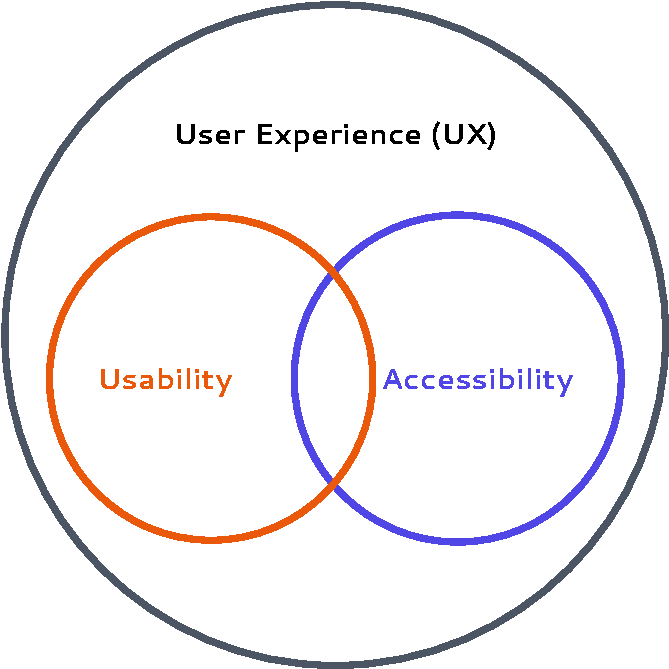
\includegraphics[height=8cm, keepaspectratio]{Accessibility_Usability_UX_Diagram}
    \caption{Relation between Accessibility, Usability, and \gls{ux}.}
    \label{fig:hsie-relations}
\end{figure}

\subsection{Benefits}
\label{Literature-HSIE-Benefits}

\textcite{Juergen_et_all_2020} point to their earlier research results that indicate implementing Accessibility on the web could provide benefits to users other than the usual primary target of Accessibility enhancements - disabled users \parencite{Schmutz_Sonderegger_Sauer_2016, Schmutz_Sonderegger_Sauer_2017, Schmutz_Sonderegger_Sauer_2018}.
This notion is seconded by \textcite{Vanderheiden_2000}, who mentions that others in similar challenging situations can benefit from Accessibility as well.
\textcite{Edyburn_2010} provides terminology identifying these two groups of users: primary and secondary beneficiaries. Specifically in the educational setting, \textcite{Edyburn_2021} mentions that Accessibility can improve the ability to use the software for both primary beneficiaries - disabled students - and secondary beneficiaries - all other students.

Examples of secondary beneficiaries concerning the web are mentioned by \textcite{WAI_Intro}:

\begin{itemize}
    \item people using different devices with smaller screens or "different input modes" \parencite{WAI_Intro},
    \item people challenged by limitations introduced by ageing,
    \item temporarily limited people - e.g. by a "broken arm or lost glasses [...or a] bright sunlight" \parencite{WAI_Intro}, or conditions that do not allow audio playback,
    \item and people limited by their internet connection - i.e. latency or bandwidth.
\end{itemize}

However, \textcite{Juergen_et_all_2020} also mention that benefits from some specific concepts could be limited. For example, "using easy language" \parencite[p. 1210]{Juergen_et_all_2020} was shown to have limited benefits and considerable disadvantages like decreased enjoyment and higher required time to consume the content \parencite{Schmutz_Sonderegger_Sauer_2019}.

As for the Usability and \gls{ux} benefits, as was already mentioned in \autoref{Literature-HSIE-Definition}, these can be used as a competitive advantage \parencite{Wegge_Zimmermann_2007}, or, more specifically, to improve some metric like conversion rate, traffic numbers, user performance, or usage of key features \parencite{Nielsen_2008}.
Surveys summarised by \textcite{Nielsen_2008} indicate a high, double-digit \gls{roi} even though this number is declining year on year, presumably due to the ever-improving starting state.

\subsection{Implementation}
\label{Literature-HSIE-Implementation}

\subsubsection{Accessibility}

According to \textcite[p. 296]{Wegge_Zimmermann_2007}, there are three main approaches when implementing the Accessibility requirements:

\begin{itemize}
    \item Universal Design - designing software to be usable without any modifications by the widest range of users.
    \item Adaptive Design - designing software to be adaptable to different types of users.
    \item Interoperability with Assistive Technology - designing software to work with existing assistive software.
\end{itemize}

\textcite{Wegge_Zimmermann_2007} warn about the downsides of Universal Design: the ability to hinder the experience of the majority, stigmatisation, and implementation difficulties due to conflicting requirements.
\textcite{Juergen_et_all_2020} reiterate this point and add that a compromise may need to be made to satisfy all groups.
In contrast to that, implementation of Adaptive Design allows to opt-in to alternative, independent representations without influencing other groups of users \parencite{Wegge_Zimmermann_2007}.
Similarly, assuming the software follows the relevant standard \gls{api}, Interoperability with Assistive Technology allows selected users to use their existing tools, e.g. screen readers \parencite{Wegge_Zimmermann_2007}.
\textcite{Edyburn_2021} mentions the usefulness of Assistive Technologies like speech-to-text and text-to-speech in relation the learning environment and argues they are already available on most platforms and can be targeted at both types of beneficiaries.

\textcite{Juergen_et_all_2020} mention that the web has received a significant amount of attention in regards to Accessibility thanks to its perceived importance.
\gls{wai} is recognised as the relevant source of information used to develop and verify the Accessibility of web services \parencite{WAI_Intro}.
\gls{wcag} by \gls{wai} are adopted around the world, including by \textcite{ISO_40500:2012} and in the law \parencite{WAI_Policies}, an example of which is the \gls{eu}['s] Web Accessibility Directive \parencite{EU_Web_Accessibility}.
The current stable version is \gls{wcag} 2.1. While it is version 2.0 that is standardised in \textcite{ISO_40500:2012} and is the source for many legally binding documents, any minor versions like \gls{wcag} 2.1 are backwards compatible as they contain verbatim all requirements from the previous version \parencite{WAI_WCAG}.

\label{Kinds-of-Accessibility}
According to \textcite{WAI_Topics}, there are two kinds of Accessibility requirements: technical, which are mostly fulfilled by properly utilising available \gls{api}[s]; and interaction/visual requirements implemented with the assistance of real users.
Implementing both kinds of requirements should mean the service is both "technically and functionally usable" \parencite{WAI_Topics}.
\textcite{WAI_Topics} warns that Accessibility is ideally implemented during the development as implementing it later can be problematic, but also admits addressing all Accessibility issues is challenging even for large projects.

While Accessibility for web services can be implemented following the mentioned industry-standard \gls{wcag}, \textcite{Vanderheiden_2000} argues that implementing Usability and Accessibility, in general, can be overwhelming.
\textcite{Vanderheiden_2000} points to hundreds of strategies that one may end up choosing from without appropriate consideration.
Therefore, \textcite{Vanderheiden_2000} proposes prioritisation using four dimensions:

\begin{itemize}
    \item Accessibility - does the given feature influence the basic Accessibility of the service. Not implementing the most important ones means the service is completely unusable for some groups, while skipping the less important ones only makes the product harder to use for some groups of users.
    \item Independence - should the user independently use the feature. Less used and more involved features can be usable and delegated only to more advanced users, while everyday tasks must be usable by all.
    \item Efficiency and Urgency - how much impact does the task have on the efficiency of the given type of user, and is there some time constraint. Tasks performed very frequently and within some time constraints have a higher priority. Tasks that are not reversible and a failure can have significant consequences have a higher priority.
    \item Ease of Implementation - the estimated effort required to implement the Usability enhancement. Enhancements that are easier to implement have higher priority.
\end{itemize}

\subsubsection{Usability and \gls{ux}}

Considering a narrower definition of Usability, \textcite{Nielsen_1993} looks at Usability as a quality and mentions a service should be both usable and have utility (provide features users need).
The relation between Usability, utility and other acceptability requirements is outlined in Figure~\ref{fig:system-acceptability}.
Assuming service is Accessible and has utility, \textcite{Nielsen_1993} recognises the following five qualitative components:

\begin{itemize}
    \item Learnability - how easy a service is to pick up for the first time.
    \item Efficiency - how quickly can tasks be successfully performed.
    \item Memorability - to what extent is the efficiency reproducible after a period of time not using a service.
    \item Errors - how many errors are being made, their significance, and recovery.
    \item Satisfaction - how nice the service feels to use.
\end{itemize}

\begin{figure}[ht]
    \centering
    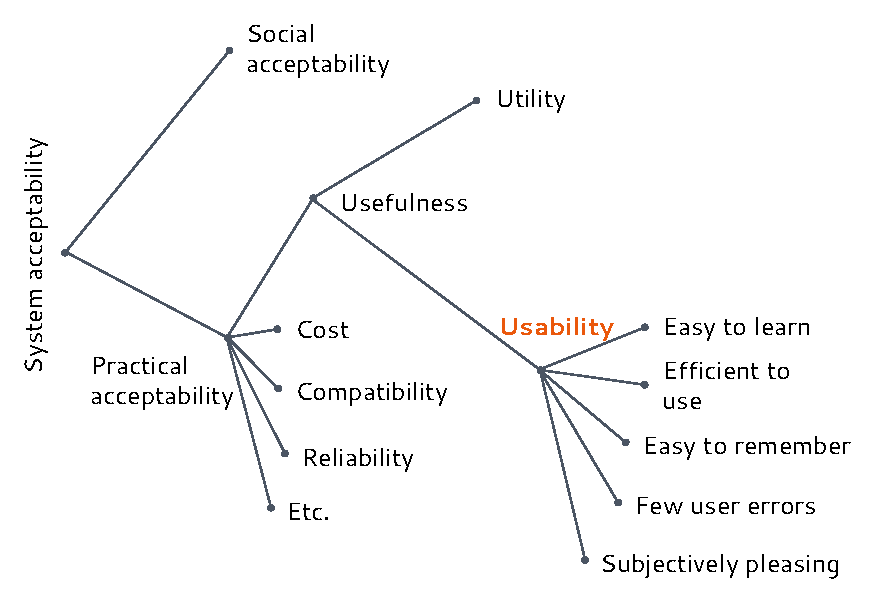
\includegraphics[height=8cm, keepaspectratio]{System_Acceptability_Map}
    \caption{Usability in the context of System Acceptability \parencite{Wilson_2009}.}
    \label{fig:system-acceptability}
\end{figure}

The \gls{cue} model introduced by \textcite{Thüring_Mahlke_2007} discerns between "instrumental" and "non-instrumental" qualities \parencite[p. 1209]{Juergen_et_all_2020}.
Similarly, \textcite{Hassenzahl_2008} distinguish between "pragmatic" and "hedonic" qualities \parencite[p. 1209]{Juergen_et_all_2020}.
Both former categories match the first four qualities mentioned by \textcite{Nielsen_1993}, while the latter are closer to Satisfaction and encompass, e.g., visual aesthetic, relatedness, or stimulation \parencite{Thüring_Mahlke_2007, Hassenzahl_2008}.

\subsection{Evaluation}
\label{Literature-HSIE-Evaluation}

\subsubsection{Accessibility}

\textcite{WAI_Evaluation} acknowledges two ways to evaluate the Accessibility of web services akin to the two kinds of Accessibility requirements outlined in \ref{Kinds-of-Accessibility}:

\begin{itemize}
    \item using tools - software can automatically check a service against standards like \gls{wcag} or assist humans but cannot solely determine whether a web service is Accessible \parencite{WAI_Evaluation_Tools},
    \item with the assistance of humans as target users - users without disabilities or with different disabilities can be involved in evaluating Accessibility but alone cannot determine whether a web service is Accessible \parencite{WAI_Evaluation_Users}.
\end{itemize}

A comprehensive evaluation of conformance to \gls{wcag} can be performed using \gls{wcagem} \parencite{WAI_Evaluation_Methodology}.
It can be used for self-assessment or assessment by a third party and can involve both tools and users \parencite{WAI_Evaluation_Methodology}.
\textcite{WAI_Evaluation_Methodology} provides the five steps that make up the \gls{wcagem}, and that can be executed with the help of \gls{wcagem} Report Tool\footnote{\gls{wcagem} Report Tool is available online at \url{https://www.w3.org/WAI/eval/report-tool}.}:

\begin{enumerate}
    \item Determine the overall scope - define the evaluated subject, baseline, and objectives, including the mentioned \gls{wcag} version and conformance level - A, AA, or AAA - with AAA being the strictest one and AA being the recommended one.
    \item Explore the subject - find what are the used technologies, e.g., HTML, WAI-ARIA, or MathML, and identify essential functionality or types of content, e.g., authentication, check-out, or blog pages.
    \item Pick sample from the subject - pick specific (random) \glspl{url} representative of the findings from the previous step or all available \glspl{url} if possible.
    \item Evaluate the sample - follow the \gls{wcag} to gather information about compliance with all of the requirements of the relevant conformance level for each identified \gls{url}.
    \item Report the results - create a report, e.g. using the provided template, that includes an executive summary, background, scope, details about the person evaluating, review process approach and goal, and results and recommendations \parencite{WAI_Evalutation_Report}.
\end{enumerate}

\begin{figure}[H]
    \centering
    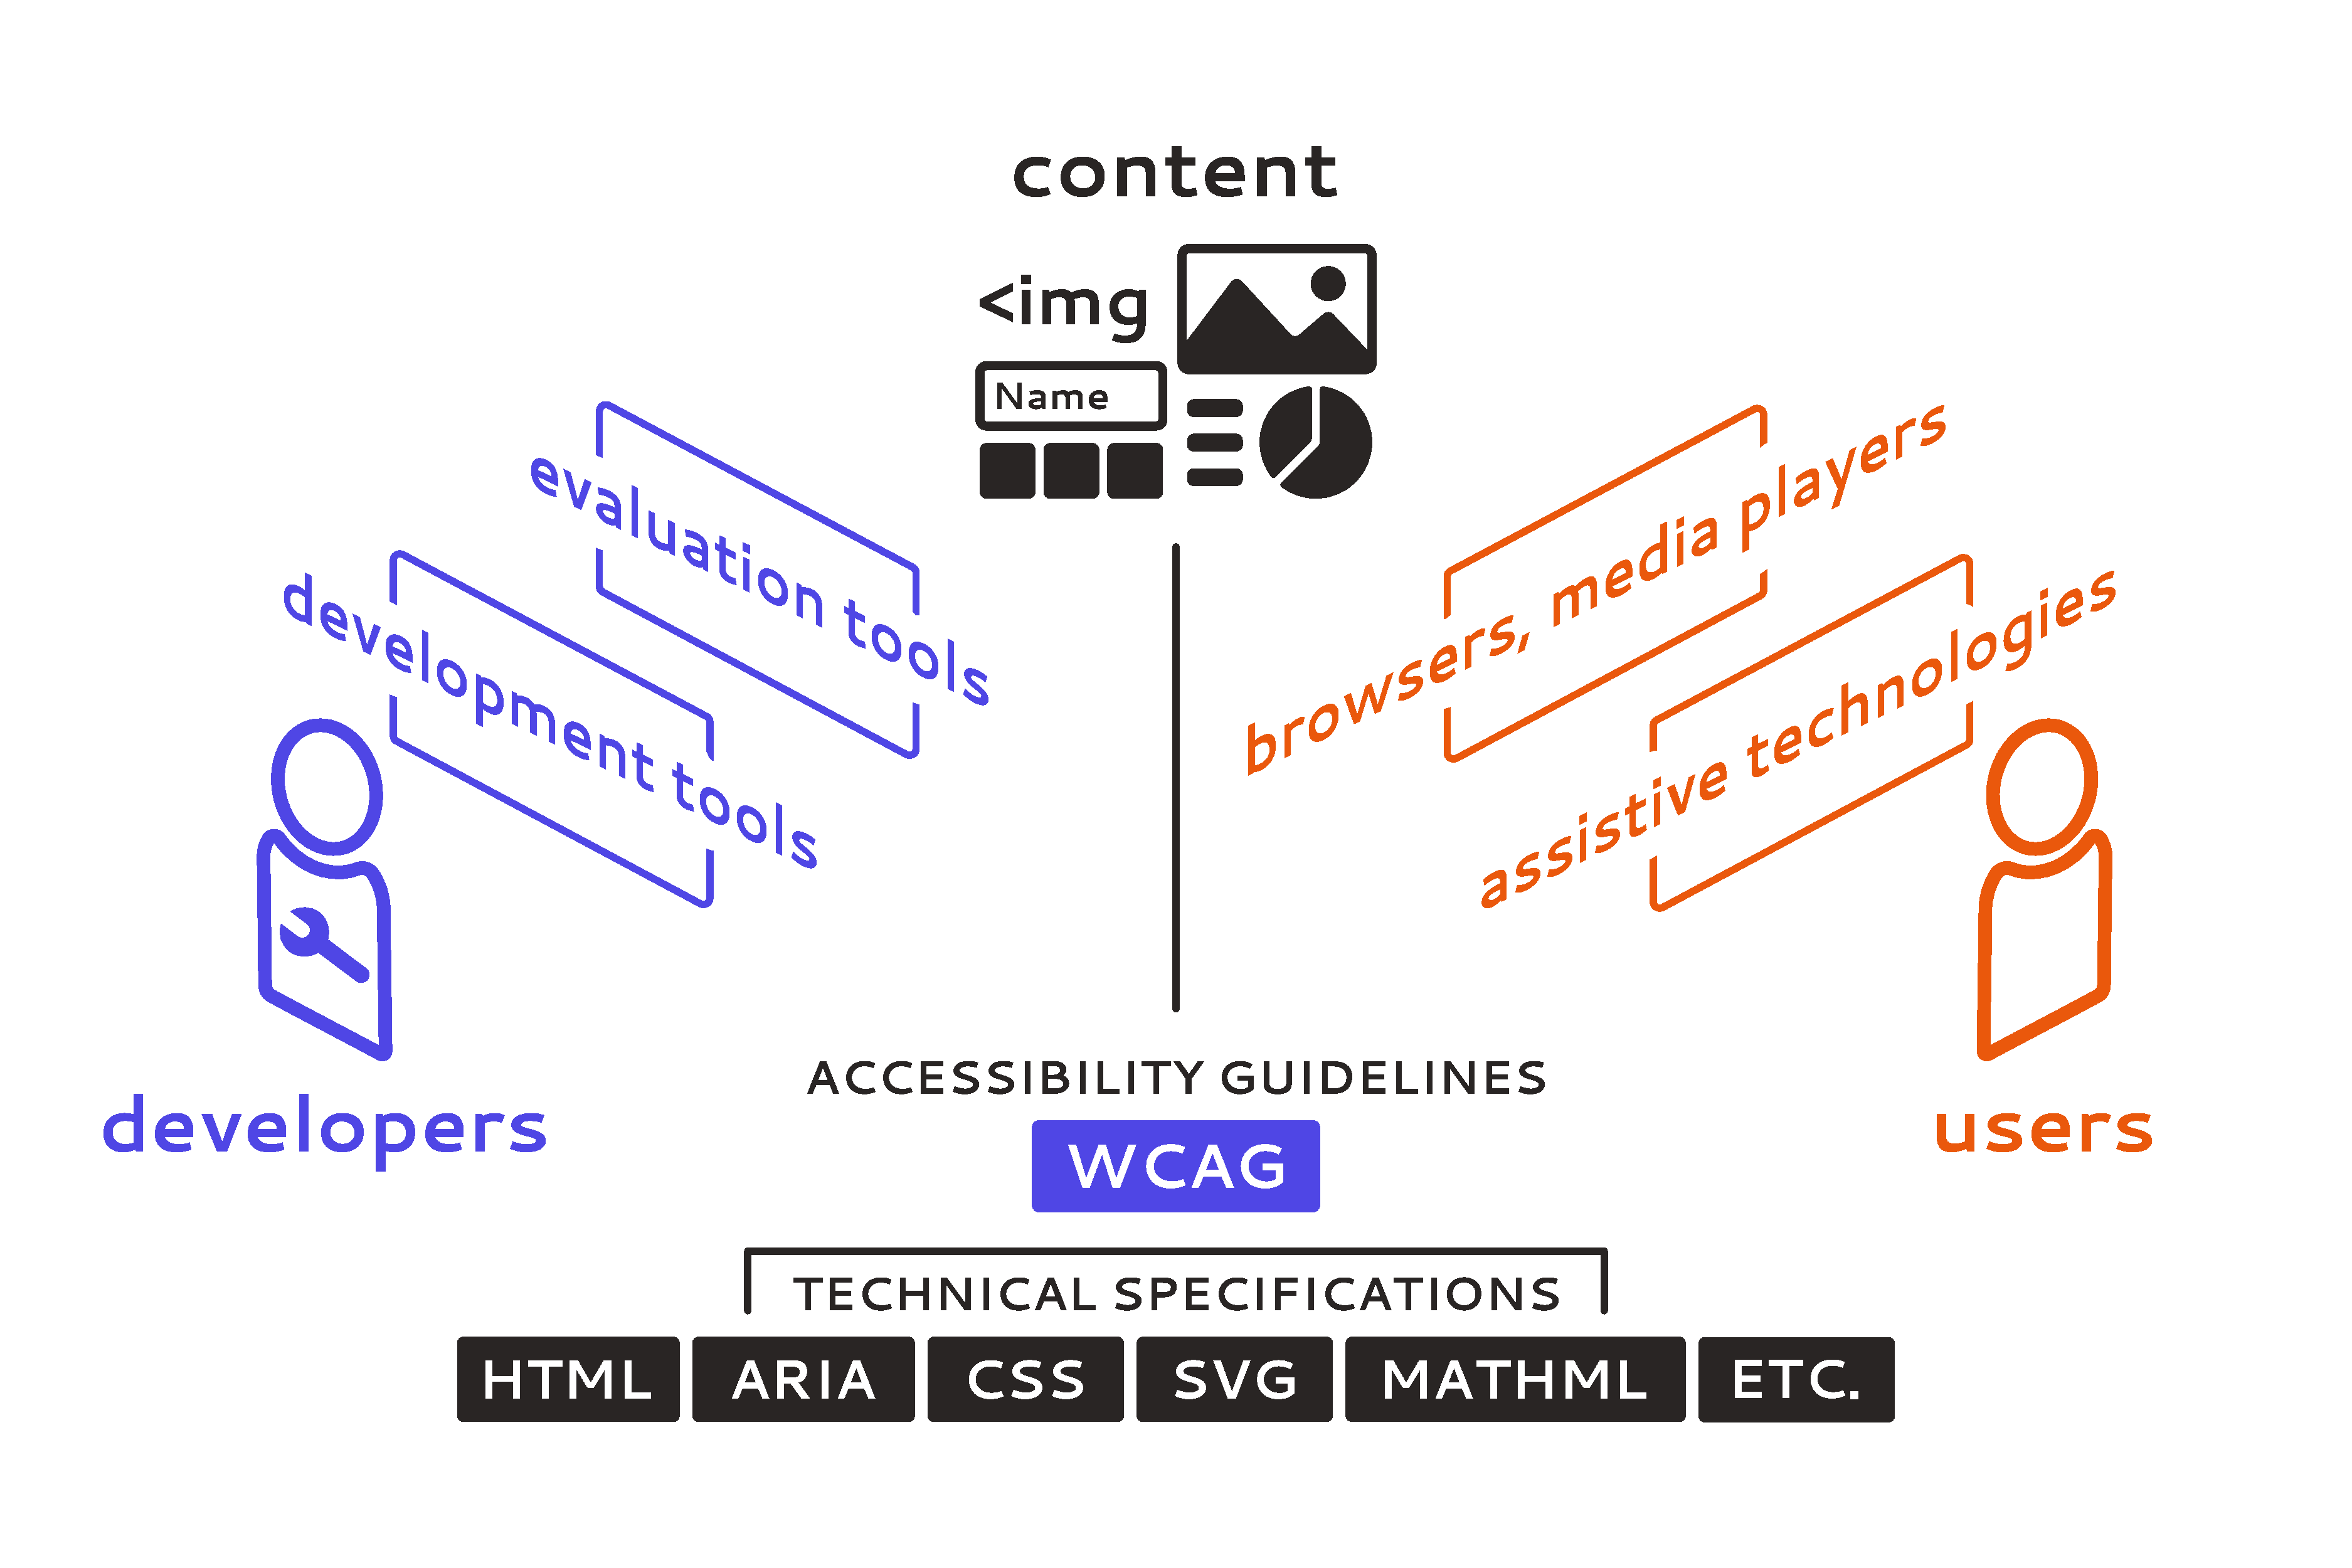
\includegraphics[height=8cm, keepaspectratio]{Accessibility_Overview_Diagram}
    \caption{Web content relation to Accessibility guidelines, users, and developers \parencite{WAI_WCAG}.}
    \label{fig:wcag-context}
\end{figure}

\label{Accessibility-Tools}

\textcite{WAI_Evaluation_Tools} mentions a wide variety of (semi) automated evaluation tools are available to cover different guidelines, languages, or technologies and working with different environments, inputs, and outputs.
Three examples of types of tools in regards to the mode of operation include \glspl{api}, browser plugins, and online services\footnote{A list of web accessibility evaluation tools maintained by \gls{wai} is available online at \url{https://www.w3.org/WAI/ER/tools}.} \parencite{WAI_Evaluation_Tools}.
Findings from \textcite{Frazão_Duarte_2020}, who reviewed the currently available most popular browser plugins, support the recommendation from \gls{wai} on the need to use multiple tools and the need to perform manual actions on top of the automated checks.
For example, the most popular one, Google's Lighthouse, based on the aXe engine, checks for 19 criteria compared to TotalValidator's 50, and it seems to be more efficient in one kind of criteria while the others are more efficient at finding errors relevant for other criteria \parencite{Frazão_Duarte_2020}.
As far as evaluation with the assistance of users is concerned, \textcite{WAI_Evaluation_Users} warns users having different backgrounds and representing different groups should be ideally involved to capture a wide variety of real potential users and to eliminate subjectivity.
\textcite{Wegge_Zimmermann_2007} reiterate Accessibility evaluation involves users from different groups that can tell whether the service can be used with their disability, is compatible with their assistive technology, or if the service behaves the way they expect.

\subsubsection{Usability and \gls{ux}}

\textcite{Wegge_Zimmermann_2007} mention that Usability, in contrast to Accessibility, is not typically tested by adherence to standards but by testing and analysing the impact on the end-users.
\textcite{Edyburn_2021} adds that we can monitor subjective measures like decreased frustration or objective measures like increased productivity.

A distinction is pointed to by \textcite{Juergen_et_all_2020}, who reiterate two kinds of Usability testing:

\begin{itemize}
    \item formative - helps pinpoint and solve problems with service during the development - called "diagnostic usability" by \textcite{Lewis_2014},
    \item summative - evaluates a service to compare it to other service or criteria - called "measurement-based usability" and told to have similarities to experimental psychology by \textcite{Lewis_2014}.
\end{itemize}

\textcite{Juergen_et_all_2020} also argue that the same thinking could be followed when evaluating \gls{ux} as well, even though such explicit distinction has not been made yet in regards to \gls{ux}.
There is a large number of concrete methods that could be utilised, like questionnaires, observation, interviews, data logging, or user testing \parencite{Juergen_et_all_2020}.
While expert-based methods are seen as more cost-effective, some argue they do not reflect real use the way user-based do, and user-based methods can generate a broader range of data \parencite{Juergen_et_all_2020}.
\textcite{Juergen_et_all_2020} argue a "principal method" to evaluate the Usability of a service is user testing - users use artefact watched by observers that acquire objective quantitative data, e.g., on efficiency or errors.
All while focusing on specific roles and tasks \parencite{Wegge_Zimmermann_2007,McCloskey_2014}.

\gls{ux} evaluation that takes into consideration emotion (i.e. not or not only Usability) is argued to be harder to evaluate since it is very individual \parencite{Juergen_et_all_2020}.
Therefore, expert-based methods are replaced by user-based methods that can be based on more broad but still subjective established questionnaires like \gls{mecue} \parencite{Juergen_et_all_2020}.
Considering another angle of subjective \gls{ux} evaluation that includes Usability, \textcite{Lewis_2014} asserts practitioners should use standardised Usability questionnaires which are proven to reliably assess perceived Usability and are referenced in national and international standards.
For example, \gls{sus} \parencite{Lewis_2018} or \gls{pssuq} \parencite{Lewis_1995, Lewis_2002}.
Both of these standardised questionnaires are available for free, should produce statistically significant data, and have a relatively low number of items - 10 for \gls{sus} and 16 for \gls{pssuq} \parencite{Lewis_2014}.
An even shorter alternative that has only slightly lower reliability ($r>0.8$ compared to $r>0.9$) and seems to produce results correlated to \gls{sus} repeatedly is \gls{umux} with four items and its shorter variant \gls{umux}[-LITE] with two items \parencite{Lewis_2014,Lewis_2018}.
\textcite{Schrepp_Kollmorge_Thomaschewski_2023} suggest that based on their findings researchers can feel confident choosing \gls{sus} or \gls{umux}[-LITE] if the main objective are Usability-focused aspects.
That is mainly thanks to the focus on the Usability aspects that makes these variants lend themselves well to professional software \parencite{Schrepp_Kollmorge_Thomaschewski_2023}.
The same cannot be said about software where the software is used for leisure as \textcite{Schrepp_Kollmorge_Thomaschewski_2023} mention only questionnaires like \gls{ueq-s} were able to capture hedonic qualities.

\label{sec:sus-evaluation}

Some questionnaires like the mentioned \gls{sus} have a long history and so can offer useful suggestions based on the data from years of use \parencite{brooke_2013}.
For example, \textcite[p. 35]{brooke_2013} points out that the word "cumbersome" used in one of the questions is not easily understood by non-native English speakers.
To address this problem, \textcite[p. 35]{brooke_2013} suggests it can be replaced with the word "awkward", citing several supporting studies.
In terms of interpreting the resulting \gls{sus} score, \textcite[pp. 36-37]{brooke_2013} points out there are data-backed ways to assign a grade and an adjective to resulting scores the way \textcite{bangor_determining_2009} and \textcite{sauro_practical_2011} did.

In relation to e-learning software, in particular, \textcite{Darin_et_all_2019} also mention that commonly used instruments are questionnaires.
That being said, \textcite[p. 60]{Darin_et_all_2019} also point to "a rising trend [of capturing both] self-reported data [and] UX measurement, in quali-quantitative approaches".
A more specific and objective alternative to capturing emotional aspects can be physiological data like body posture \parencite{Tan_Schöning_Luyten_Coninx_2013}.
However, these can come with privacy challenges and difficulties evaluating the data \parencite{Juergen_et_all_2020}.

In regards to the design of Usability testing, \textcite{McCloskey_2014} mentions that user tasks should capture key user goals, prompt users to take action, and be engaging by providing context without giving out any clues.
Remote Usability testing can, but does not have to, involve interactive sessions between user and facilitator and can be done using automated tools \parencite{Moran_2019}.
Formative Usability testing is likely to be qualitative, and even several users can identify most of the problems \parencite{Lewis_2014,Moran_2019}.
On the other hand, summative Usability testing is more likely to be quantitative and can be used to compare \parencite{Macefield_2009, Moran_2019}.

Some of the most common quantitative metrics are task success rate and time on task \parencite{Macefield_2009, Moran_2019}.
\textcite{Macefield_2009} mentions that these are suitable for analysis using statistical methods and can be used to make important decisions like go/no-go for new systems.
When processing time on task data, \textcite{sauro_chapter3_2016} suggest using geometric mean, rather than mean or median, as it seems to have a considerably lower error and bias on smaller sample sizes ($n < 25$).
However, when comparing two systems, \textcite{sauro_chapter5_2016} do not think it is worth it to use geometric mean as "two-tailed paired $t$-test is widely considered robust to violations of normality".

\textcite{Lewis_2014} contends there is no universal number of participants for summative studies, and one should try to utilise available tools to calculate the required number of participants.
\textcite{Macefield_2009} mentions that a comparative study is essentially a hypothesis test where the aim is to collect evidence a software A has better Usability metrics than software B.
As such, it is important to ensure the results are statistically significant by having a low probability ($p \leq 0.1 $, ideally $p \leq 0.05 $) of the \textit{null hypothesis} \parencite{Macefield_2009}.
Since increasing the number of participants should lower this probability, \textcite{Macefield_2009} suggests one can run the study until statistical significance is reached or the test fails.
Based on the previous data across the field, \textcite{Macefield_2009} hints that a study group should not be smaller than eight participants, with ten to twelve participants being likely to result in statistically significant data.
The same suggestion seems to apply specifically to questionnaires examining Usability on the web as well, with \gls{sus} achieving the "correct" conclusion 100\% of the time with twelve and more participants on data with a large effect size \parencite{tullis_comparison_2004}.
The relation between the sample size and the probability a "correct" conclusion is reached involving different questionnaires can be seen in Figure~\ref{fig:hsie-questionnaire-sample-size}.

\begin{figure}[H]
    \centering
    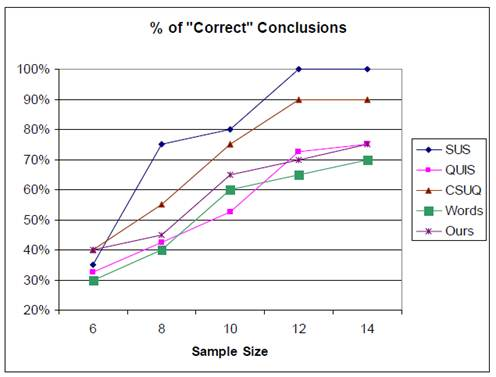
\includegraphics[height=8cm, keepaspectratio]{Sample_Size_Correct}
    \caption{Sample size vs "correct" conclusions \parencite{tullis_comparison_2004}.}
    \label{fig:hsie-questionnaire-sample-size}
\end{figure}

\textcite{Macefield_2009} mentions that the size of the effect has a strong influence on the required number of participants, and \textit{power analysis} can be done at different stages to verify the sample size required for statistically significant data or significance in general.
However, \textcite{Dziak_Dierker_Abar_2020} argue that using power analysis to decide significance during or after the study (post hoc) should never be done.
Alternatives suggested by \textcite{Dziak_Dierker_Abar_2020} for this purpose are \textit{confidence intervals} and \textit{Bayesian analysis}.
That being said, \textcite{Dziak_Dierker_Abar_2020} admits Bayesian analysis is not yet very commonly understood.
\textcite{sauro_chapter5_2016} concur with the use of confidence invervals when comparing \gls{sus} scores or time on task times.
If a between-subjects comparison is performed, \textcite{sauro_chapter5_2016} suggest the use of two-sample $t$-test to take into consideration both variation within the group and between the groups.
The relevant formula can be seen in Figure~\ref{fig:hsie-two-sample-t-test}, where $\hat{x}_1$ and $\hat{x}_2$ are means of data for system 1 and 2, $s_1$ and $s_2$ are respective standard deviations, and $n_1$ and $n_2$ are respective sample sizes.

\begin{figure}[H]
    \[ t = \displaystyle\frac{\hat{x}_1-\hat{x}_2}{\displaystyle\sqrt{\frac{s^2_1}{n_1}+\frac{s^2_2}{n_2}}} \]
    \caption{Two-sample $t$-test formula \parencite{sauro_chapter5_2016}.}
    \label{fig:hsie-two-sample-t-test}
\end{figure}

The confidence interval can then be calculated using formula in Figure~\ref{fig:hsie-confidence-interval-diff}, where $t_a$ is "the critical value from the $t$-distribution for the specified level of confidence and degrees of freedom" \parencite{sauro_chapter5_2016}.

\begin{figure}[H]
    \[ (\hat{x}_1-\hat{x}_2) \pm t_a\displaystyle\sqrt{\frac{s^2_1}{n_1}+\frac{s^2_2}{n_2}} \]
    \caption{Confidence interval formula \parencite{sauro_chapter5_2016}.}
    \label{fig:hsie-confidence-interval-diff}
\end{figure}


\section{Learning Computing Principles}

The goal of the following section is to explore the state of remote learning and \glspl{mooc} in general concentrating on the problems or potential challenges, the most popular content available for learning low-level computing principles, and its supporting software.
Learning low-level computing principles, in this case, means introduction to topics like logic gates, chip design, computer architecture, or low-level code.
The assumed demographic is senior secondary or postsecondary students, computing professionals without a formal background in computer science, or the general public interested in computers.

\subsection{State of Remote Learning and MOOCs}
\label{sec:learning-state}

Data gathered by the \textcite{us_doe_digest_2021} show roughly 60\% of U.S. postsecondary students took at least some of their classes online in 2021.
While this number is down from the COVID-19 pandemic level of 75\% in 2020, it shows a clear upward trend compared to 36\% in 2019 and 25\% in 2012 \parencite{us_doe_digest_2021}.
More broadly, the global remote learning market was valued at about 300 to 400 billion U.S. dollars in 2022 and is expected to grow at about 10\% \gls{cagr} by some market research companies \parencites{GlobalElearning_GIA_2023}{GlobalElearning_GMI_2023}.
One of the largest \gls{mooc} providers, Coursera, reported the total number of registered users grew 61\% \gls{yoy} during the pandemic year of 2020 and 30\% the year after that \parencite{Coursera_Impact_2021}.

The effects of the accelerated widespread shift to remote learning were especially apparent during the onset of the pandemic that, at one point, \textcite{UNESCO_2022} estimates caused more than a billion children ($>70\%$) to be out of the classroom globally.
\textcite{eu_covid_learning_2023} shows disadvantaged children and children in countries with lower adoption of \gls{ict} were more likely to be negatively affected.
Taking into consideration research from \textcite{tadesse_impact_2020}, these challenges were especially evident in developing countries.
\textcite{tadesse_impact_2020} point out the lack of stable internet connection and devices suitable for remote learning as some of the challenges.
In order to support all learners, \textcite{Ali_2020} mentions, among else, that it is necessary the content is "available on a wide variety of devices and mobile friendly" and accessible despite limited bandwidth or even offline.

Although remote learning has seen a major uptick in students, \gls{mooc} dropout rates can be up to 90\% \parencite{goopio_mooc_2021}.
Common problems with \glspl{mooc} leading to a high rate of dropouts include lack of time, difficulty, and bad past experience (including technical problems) with MOOC platforms \parencite{onah2014dropout}.
\textcite{goopio_mooc_2021} mention several software-related recommendations based on their systematic review of research focused on dropouts:

\begin{itemize}
    \item Increase interactivity by providing activities like quizzes, games, or video interactions.
    \item Improve course design by using smaller chunks of content with visualisation of abstract content and real examples.
    \item Use various media formats and ensure accessibility from mobile devices and with limited internet connectivity.
\end{itemize}

From the viewpoint of teaching institutions, MOOCs are said to require significant time to both create and integrate \parencite{stikkolorum2014mooc}.
That being said, \textcite{stikkolorum2014mooc} mention the use of MOOCs for software engineering education within higher education is argued to broaden student knowledge and is successfully integrated by some universities into their courses and programmes.
Furthermore, data from the \textcite{us_doe_digest_2021} show that, at least in the U.S., online classes serve a considerably higher number of racially diverse students compared to conventional classes.

\subsection{Low-Level Computing Principles}
\label{sec:learning-principles}

One of the most popular, if not the most popular, learning materials for learning computing principles is the Nand2Tetris, "taught at 400+ universities, high schools, and bootcamps", which explains how to build a computer from individual logic gates to a working virtual computer \parencite{nand2tetrisweb}.
In the process, \textcite{nand2tetris} cover a wide variety of computing principles via practical projects:

\begin{enumerate}
    \item Construction of simple Boolean gates.
    \item Design of more advanced 16-bit chips.
    \item Incremental construction of an \gls{alu} starting with simpler chips like incrementer or half and full adder.
    \item Introduction of a clock to chips and construction of registers and \gls{ram}.
    \item Programming using simplified assembly.
    \item Construction of the final computer utilizing previously built parts.
    \item Writing of an assembler that translates custom assembly language into binary runnable on the built computer.
\end{enumerate}

The learning material is offered as a book written by \textcite{nand2tetris}, as a \gls{mooc}\footnote{Available at \url{https://www.coursera.org/learn/build-a-computer}}, and in a PDF format\footnote{Available at \url{https://www.nand2tetris.org}}.
The latter is available freely under a Creative Common Attribution-NonCommercial-ShareAlike 3.0 Unported License.
However, it does not contain additional material that builds on the mentioned projects and adds more software-related topics revolving around a Jave-like Virtual Machine, a custom high-level programming language and a standard library for a custom \gls{os}.
Regardless of which form of learning material learners choose, they are expected to use the accompanying desktop Java software\footnote{Available at \url{https://www.nand2tetris.org/software}}.

Edybrun (2021) argues the industry now focuses on web-based curricula as the web already has essential accessibility tools, and frameworks like Depth of Knowledge (DOK) lend themselves better to the web environment.
More specifically, Edybrun (2021) takes note of the development of more interactive experiences than just "text on a screen" adapted from textbooks.
For example, web-based curricula can contain interactive "embedded supports", and Edybrun (2021) mentions these should be context-sensitive.
However, the only kind of examples Edybrun (2021) provides are a tool that provides a breakdown and planning of subtasks and "virtual pedagogical agents" similar to virtual assistants like Alexa or Siri but specific to the pedagogical environment.

The recently created web-based WepSIM \parencite{garcia2019wepsim} provides microdesign, microprogramming and assembly language educational simulator and was implemented by authors as an interactive way to practice learned concepts.
Compared to Nand2Tetris, which takes a more broad approach and goes through many concepts throughout several layers of abstraction, WepSIM is focused only on a thorough simulation of the CPU and instruction processing.
\textcite{garcia2019wepsim} argue the introduction of WepSIM increased the percentage of students taking the final exam and improved grades in assembly and microprogramming exercises.
\textcite{garcia2019wepsim} also add that WepSIM is usable not only as a supplementary tool but also as a standalone learning tool thanks to the bundled examples and help material.
Notably, \textcite{garcia2019wepsim} mention students were able to use WepSim on a wide variety of devices and operating systems, from Windows-NT, Linux, and macOS to Android, iOS, and Windows-Phone.


\section{Device Type Usage}
\label{sec:device-types}

The following section focuses on the current device type usage and possible trends both in developed and developing countries.
The aim is to look at statistics both among the general population and in the education sector.
Web clients are of particular interest due to the focus of this thesis.
This section is broken down into two sub-sections for developed and developing markets, as the gathered data are considerably different.

Globally, mobile devices account for around 56\% of browser market share, up from only 11\% in 2012 \parencite{StatCounter_2023}.
The shift to mobile devices slowed significantly around the year 2017, when they reached a market share of 52\%, and there has been no apparent significant change in data since then \parencite{StatCounter_2023}.
Tablet devices, on the other hand, seemed to have reached a peak of almost 7\% in 2014, and their market share has been steadily declining since \parencite{StatCounter_2023}.

In terms of \gls{os} and screen resolution, the market is now also very fragmented \parencites{StatCounter_OS_2023}{StatCounter_Resolution_2023}.
While in the past, just 10 years ago, Windows had a commanding position, now no \gls{os} has majority of the market share and the top four makes up the same market share as Windows alone did in 2009 \parencite{StatCounter_OS_2023}.
\textcite{StatCounter_Resolution_2023} also shows how there is no major screen resolution with a market share larger than 10\% the way it used to be and how the variety of screen resolutions has been growing over time.

\subsection{Developed Countries}

Contrary to the global web traffic data, data for Europe and North America still show a gradual increase in the mobile device market share with parity reached just within the last few years \parencites{StatCounter_Europe_2023}{StatCounter_NorthAmerica_2023}.
Notably, Chromebooks haven seen a considerable growth in North America and Western Europe and accounted for the majority of the upcoming learners from US K12 market in years 2020 and 2021 \parencite{Boreham_2019, IDC_2021}.
However, tablet and Chromebook shipments have since slowed down noticeably \parencite{IDC_2022}.

In terms of internet smartphone dependency, about 15\% of U.S. adults - up from 8\% in 2013 - report a mobile device is the only way they access the internet \parencite{Pew_Research_2021}.
Importantly, this group is made up mostly of the 18-29 age group and that is the only age group where we can see a clear trend of increasing smartphone dependency \parencite{Pew_Research_2021}.
That being said, looking for example at data from \textcite{Educause_2022} collected at University of Central Florida show smartphone use for learning has not increased during the years 2016-2021 with laptops still dominating.

\subsection{Developing Countries}

In sharp contrast to Europe and North America discussed before, developing markets like Africa and Asia have a much higher market share of mobile devices at about 70\% \parencites{StatCounter_Africa_2023}{StatCounter_Asia_2023}.
Additionally, mobile devices overtook desktop devices much sooner, around the year 2015 \parencites{StatCounter_Africa_2023}{StatCounter_Asia_2023}.
As far as tablet devices go, there is no considerable difference we can observe with developing markets \parencites{StatCounter_Africa_2023}{StatCounter_Asia_2023}.

Similarly, while developed countries were seeing noticeable growth in Chromebook and tablet shipments, developing countries did not \parencite{Boreham_2019}.
Internet smartphone dependency is very high in emerging economies, with only about 34\% of households having access to a desktop, laptop, or tablet device \parencite{Pew_Research_2019}.
Importantly, this number varies greatly between individual developing countries, with India being at the lower end with just 11\% and Lebanon being at the high end with 57\% \parencite{Pew_Research_2019}.
That being said, smartphone ownership is prevalent mainly in the age group of 18-29, with typically less than 40\% of people aged 50+ owning a smartphone in developing countries \parencite{Pew_Research_2019}.
As far as use in education goes, data seem harder to find, but surveys say the majority of people think smartphones have a positive impact on education and educated people are more likely to own smartphones \parencite{Pew_Research_2019}.


\section{Text and Code}
\label{sec:text-code}

This section starts with a look at the text as a learning material that humans produce and consume, continues with a production of a source code from the viewpoint of a learner, and ends with a short subsection on how the code is processed by a machine.

\subsection{Producing Learning Material}

For the purposes of this thesis, we can simplify the choice of a way to produce learning material by considering two approaches:

\begin{enumerate}
    \item \gls{wysiwyg} editors like Microsoft Word and PowerPoint or Adobe Dreamweaver and Captivate.
    \item Plain text formats like \LaTeX, HTML, or Markdown and the tools that are necessary to make them usable.
\end{enumerate}

The first group of tools is commonly mentioned when presenting authoring tools for learning content \parencite{khademi_review_nodate}.
While most of these tools are said to be easy to use and often concentrate on creating courses, the majority of them are also paid, and there are concerns about interoperability \parencites{khademi_review_nodate}{shieber_why_2014}.
One particular concern mentioned by \textcite{shieber_why_2014} is the lack of output consistency when different users use the large range of functionality of these tools differently.

Compared to the problems with the input of \gls{wysiwyg} editors mentioned above, plain text input is by nature backwards compatible and interoperable as it is largely a UTF-8 encoded text \parencite{shieber_why_2014}.
However, the complexity of plain text formats can differ considerably.
LaTeX, which is used extensively within the scientific community, is commonly understood to be more powerful and complex, carries larger overhead on the input, and can potentially take longer to write \parencites{baramidze_latex_2013}{knauff_efficiency_2014}{shieber_why_2014}.
One of the most common specifications of Markdown, Commonmark, features a two-page long self-explanatory reference guide\footnote{Available at \url{https://commonmark.org/help/}.} while LaTeX distributes a 31-page long user guide\footnote{Available at \url{https://www.latex-project.org/help/documentation/usrguide.pdf}.}.
Moreover, Markdown is said to have a lower overhead than both LaTeX and \gls{html} \parencite{shieber_why_2014} while still permitting extensibility with LaTeX-like features \parencite{shieber_why_2014} and allowing for potentially better accessibility \parencite{voegler_markdown_2014}.
The output format LaTeX and Markdown focus on seems clear from the respective websites.
While the LaTeX project website\footnote{Available at \url{https://www.latex-project.org}.} commonly mentions PDF as the output format, Commonmark specification\footnote{Available at \url{https://spec.commonmark.org/0.30/}.} directly mentions \gls{html} as the expected output.
\gls{html} output is possible with LaTeX as well, but the efficiency of the most commonly used tool\footnote{LaTeX2HTML available at \url{https://www.latex2html.org/}.} is limited as the produced \gls{html} is said to be often substandard \parencite{voegler_markdown_2014}.

\subsection{Writing Code}
\label{sec:writing-code}

According to a survey conducted by \textcite{StackOverflow_2023}, more complex \glspl{ide} like Visual Studio Code, Visual Studio, or IntelliJ IDEA are used by more developers than simpler text editors like Notepad++ or Vim.
The most popular \gls{ide} used by more than 70\% of professionals and learners is Visual Studio Code \parencite{StackOverflow_2023}.

Research focusing on the ease of use of sophisticated \glspl{ide}, especially among learners, is inconclusive.
While a survey from \textcite{owoseni_2016} suggests learners find sophisticated \glspl{ide} difficult to use when learning programming, \textcite{vihavainen_how_2014} use session traces to back the opinion there is no evidence learning to use an \gls{ide} is hard.

As far as a web-based \gls{ide} goes, \textcite{valez_student_2020} explored the idea of using a pre-configured custom \gls{ide} that is a low-threshold alternative to common \glspl{ide}.
While most participants found the web \gls{ide} useful and found the fact that it was web-based and did not require installation useful, it was also found to often lack the functionality learners were looking for and was used mostly by more junior students \parencite{valez_student_2020}.

\subsection{Parsing Code}

This subsection starts with a mention a subset of basic graph terminology relevant for this thesis and some basic algorithms and graph properties.
After a brief introduction to graph theory, it is possible to talk about tokenizers and parsers from a practical point of view of a software developer.

\subsubsection{Graph Theory}

A graph is a data structure that consists of a non-empty finite set of \emph{vertices} and a possibly empty finite set of \emph{edges} \parencite{wilson_graph_2009}.
Each edge connects exactly two vertices, and if the edges have a direction, we call the graph a \emph{directed} graph \parencite{wilson_graph_2009}.

There are many different ways how to traverse a graph.
One such way is to use the \gls{bfs} algorithm.
\gls{bfs} follows the following logic \parencite{wilson_graph_2009}:

\begin{enumerate}
    \item Take a vertex \emph{v}.
    \item Visit all vertices that have an incoming edge from \emph{v}.
    \item Repeat step 1. with the least recently visited \emph{v} from which we did not yet visit other vertices.
\end{enumerate}

If we can find a path through the graph that starts and ends with the same vertex, it is said it contains a \emph{cycle} \parencite{wilson_graph_2009}.
In case some vertex has no associated edges, it is an \emph{isolated vertex}, and if it is not possible to visit all vertices via edges from each vertex, the graph is called \emph{disconnected} \parencite{wilson_graph_2009}.
Figure~\ref{fig:text-graph-basics} shows an example graph that is disconnected as there is no edge connecting $J$ with the rest of the graph.
Additionally, it is cyclic, as vertex $DF$ creates a cycle that could be removed by removing one of the edges $DE$, $EF$, or $DF$.

\begin{figure}[H]
    \centering
    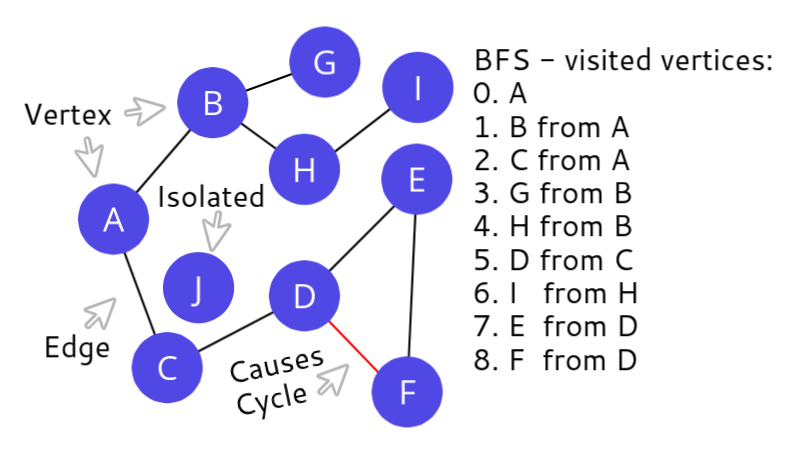
\includegraphics[width=380pt, keepaspectratio]{Graph_Basics}
    \caption{Example disconnected graph showing different concepts.}
    \label{fig:text-graph-basics}
\end{figure}

A graph is considered a \emph{tree} if it has exactly one path between any of the vertices, does not contain cycles, and is not disconnected \parencite{wilson_graph_2009}.
A tree is called \emph{rooted} if exactly one vertex is chosen as the root and all edges are "directed away from the root" \parencite{Baek_trees_2015}.
Figure~\ref{fig:text-tree-basics} shows an example of such a tree.
Vertices that have at least one outgoing edge are called \emph{internal vertices}, while vertices that have no outgoing edge are called.
\emph{Children} of an internal vertex are all vertices that have an incoming edge from that internal vertex \parencite{Baek_trees_2015}.

\begin{figure}[H]
    \centering
    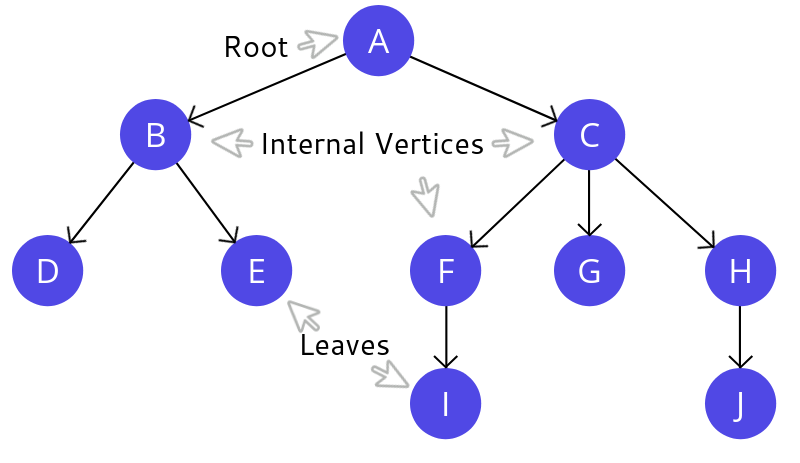
\includegraphics[width=380pt, keepaspectratio]{Tree_Basics}
    \caption{Example directed rooted tree.}
    \label{fig:text-tree-basics}
\end{figure}

\subsubsection{Tokenizers and Parsers}

\todo[inline]{Is referencing fine here? How to cite sources if I've only loosely used \parencites{tomassetti_parsing_2017}{Kjolstad_parsing_2023} as most of the literature is too theoretical and "unwieldy"?}

Parsing is a process of turning a text in a given \emph{language}, like code, into some meaningful object, for example, a program that can be executed \parencites{tomassetti_parsing_2017}{Kjolstad_parsing_2023}.
A naive approach to parsing is to go through the program character by character using a loop.
However, the logic of our language, called \emph{grammar}, would have to be captured within the procedural code, which would make it rather verbose, inflexible, and relatively hard to understand.
Instead, the grammar of the language is commonly defined separately and serves as an input for a \emph{parser generator}, which creates the parser.
The parser can operate on individual characters, in which case it is said to be \emph{scannerless} as it lacks a \emph{scanner} that would pre-process the text.
The scanner groups individual characters into more meaningful tokens and, for the purposes of this thesis, is also referred to as \emph{lexer} or \emph{tokenizer}.

Therefore, we can say processing of the text on the input goes through three distinct consecutive phases:

\begin{enumerate}
    \item \textbf{Lexing}: A string of characters on the input is broken down using a lexer into a string of tokens.
    \item \textbf{Parsing}: A string of tokens on the input is turned into a \gls{cst} using a parser - if the input is valid.
    \item \textbf{Processing}: A valid \gls{cst}, which is mostly just a set of tokens represented using a tree, is simplified into an \gls{ast}, which is a convenient logical representation of the described object.
\end{enumerate}

From a practical point of view, lexing is typically done using regular expressions as it is the simplest sufficient way to define a regular language used for tokens.
Moreover, the processing of parsed tokens can usually be done during the parsing, rather than after, skipping the extra tree traversal.
Therefore, parser generators can take: 1. one or more regular expressions defining tokens, 2. grammar, and 3. processing rules on the input and produce encapsulated parser abstraction capable of performing all three mentioned steps.
As such, the produced parser takes text on the input and provides the \gls{ast} on the output.

Since the job of a lexer and parser generator is rather generic, these are abstracted away by a library or a set of libraries.
The specification of grammar is left to a human, and the supported features differ between different types of parser generators.
A commonly used feature is recursion within the grammar rule.
A special case is a left and right recursion when the rule refers to itself on the leftmost or rightmost part of the rule.

Whether a given grammar can be written concisely and the performance of the generated parser is sufficient are typical deciding factors when choosing a parser generator.
Conciseness allowed by using features like left and right recursion may require a higher complexity that can mean a worse performance depending on the use case.
Simpler and faster parsers called \emph{LL} parse from left to right and produce a tree from the largest logical blocks to the smallest logical blocks called \emph{terminals}.
More flexible but potentially slower are parsers using the \emph{Earley} algorithm.
Earley algorithm uses top-down dynamic programming and enables support of both left and right recursion, and allows for ambiguous grammar.
While the average performance of an Ealery parse is $\theta(n^3)$, where $n$ is the number of tokens on the input, there are multiple ways to achieve better performance (and complexity class): by using left recursion, by using unambiguous grammar, or by using an implementation that features optimizations from \textcite{leo_general_1991} if using right recursion in an LL grammar.


\section{Creating Open Web Application}
\label{sec:creating-application}

Taking into account the vehicle of this research is an open web application that takes inspiration from an existing tool and reuses various open content, this section starts with the exploration of legal basis.
Then, it looks at some basic necessities of open software to improve chances the software succeeds.
Afterwards, it covers the most relevant software engineering topics regarding the development and deployment, reliability and security, and testing, that are used later in the thesis.

\subsection{Legal Background}

The following subsection deals with the legal matter required for someone who produces software that is based on an existing work and is assumed to be similarly reused again.
Moreover, it looks specifically into exclusions of the copyright law and, even more specifically, law relevant to the reuse of Nand2Tetris mentioned in \autoref{sec:learning-principles}.

\subsubsection{Free Versus Open}

In relation to software, there are two ways to define "free" \parencite[Chapter~1]{Fogel_2022}.
The first definition most people think of is free as in "zero-cost" \parencite[Chapter~1]{Fogel_2022}.
The second definition, on the other hand, deals with "the freedom to run, copy, distribute, study, change and improve" \parencite{FFS_2023}.
Because of the ambiguity of the English language in this case, an alternative way to refer to the software that follows the second definition is to call it an \gls{oss} \parencite{Fogel_2022}.

\subsubsection{Licensing}

There are significant legal implications of licensing both when producing and consuming third-party software and other assets \parencites[Chapter~9]{Fogel_2022}[pp. 11-12]{Duras_2020}.
The range of licenses one can apply or come across is rather wide, but the main aspect relevant to this thesis is the "openness" - to what extent one can apply the mentioned freedoms.
As the author summarised before in \textcite{Duras_2020}, we can group these into three categories:

\begin{itemize}
    \item \textbf{Proprietary}: The least open. Under the complete control of the author, usually confidential and paid.
    \item \textbf{Copyleft Open Source}: Technically open. Users have all the mentioned freedoms. However, they are severely restricted in how they can modify and distribute software. The modified work must be licensed under a compatible Copyleft license - i.e. not proprietary or permissive - and changes often have to be tracked. While it is considered a desired feature, it also greatly influences reuse.
    \item \textbf{Permissive Open Source}: The most open. Users have all the mentioned freedoms. Licenses are usually very short and do not place any restrictions - the users are free to do whatever they want as long as the author is attributed, not held liable for damage, and it is clear what was the original license.
\end{itemize}

\begin{figure}[H]
    \centering
    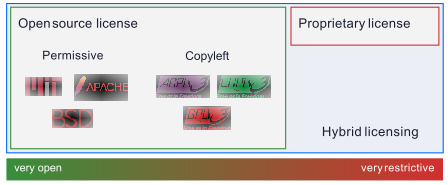
\includegraphics[width=380pt, keepaspectratio]{License_Comparison}
    \caption{License type comparison and examples \parencite{Duras_2020}.}
    \label{fig:license-comparison}
\end{figure}

While the above-mentioned licenses are commonly used to license software, one notable group of licenses commonly applied to other creative works are the \gls{cc} licenses \parencite{Hagedorn_2011}.
These can differ considerably in restrictions they impose on users, from just requiring attribution - \gls{cc} BY\footnote{Available at \url{https://creativecommons.org/licenses/by/4.0/}.} - through disallowing commercial use and mandating the use of the same license - \gls{cc} BY NC SA\footnote{Available at \url{https://creativecommons.org/licenses/by-nc-sa/4.0/}.} - to even prohibiting any adaptation - \gls{cc} BY NC ND\footnote{Available at \url{https://creativecommons.org/licenses/by-nc-nd/4.0/}.} \parencite{Hagedorn_2011}.
As such, they move almost across the whole spectrum of "openness" outlined in Figure~\ref{fig:license-comparison}.
The non-commercial variant is especially controversial as there are differing opinions on what constitutes commercial use \parencite{Hagedorn_2011}.
While for-profit companies using a specific creative work to generate profit are a clear case of commercial use, a work by non-commercial organizations or individuals that is not directly compensated may or may not be classified as commercial use \parencite{Hagedorn_2011}.

\subsubsection{Copyright Exclusions}

In relation to software, there are some aspects that may not constitute a copyrightable work.
A common requirement for work to be copyrightable is for it to be original \parencite{Fisher_2016}.
While the level of originality (creativity) required in the \gls{us} or Japan is considered to be low, within the \gls{eu}, it is higher \parencite{Fisher_2016}.
Under the \gls{eu} law, the work "must reflect the author's own intellectual creation" and the author must be able to make their own choices \parencite[p. 443]{Fisher_2016}.
The latter alludes to external limitations - like when the author has to make certain choices to ensure interoperability \parencite{Fisher_2016}.

Specifically for programming languages, \textcite{Rose_2012} mention the ruling of \gls{eu}'s highest court that confirmed the "functionality [...] nor the programming language and the format of data files [...] constitute a form of expression [... and so ...] are not protected by copyright [...]" \parencite{cjeu_2012}.
Moreover, it is allowed "to observe, study or test the functioning of that program so as to determine the ideas and principles" \parencite{cjeu_2012}.
It is based on the argument that any other decision would go against the "necessary innovation and competition" \parencite{Rose_2012}.
However, it was made clear this does not apply to the actual source code, object code, or the supplied manual \parencite{Rose_2012}.

Israel's copyright law is thought to be originally largely influenced by British and European law, with recent influences of the more lenient approach of the \gls{us} \parencite{Greenman_2012}.
In relation to software, as is the case in the \gls{eu}, "the idea behind software is not protected by copyright" \parencite{suslina_approaches_2018}.

\subsection{Essential Steps}
\label{sec:oss-essential-steps}

\textcite[Chapter~2]{Fogel_2022} mentions the following as the first steps relevant to this thesis when creating \gls{oss}:

\begin{enumerate}
    \item \textbf{Name}: Choose a name that, among else, can be easily branded, is easy to use even for non-native speakers, and is available as a .com or .org domain.
    \item \textbf{Mission Statement}: Provide a concise description of what the software does so that the user knows "within 30 seconds" \parencite{Fogel_2022} if they are interested.
    \item \textbf{Free}: Make sure to always make it clear the software is free.
    \item \textbf{Features and Requirements}: Make it clear what the software offers and requires.
    \item \textbf{Version Control and Bug Tracking}: Use a publicly accessible place like Github to host the code and manage feature requests and bug reports.
    \item \textbf{Communication}: Provide ways for the users to communicate with the author and between themselves and keep it open and friendly.
    \item \textbf{Guidelines and Documentation}: Offer developer guidelines and (even if short) documentation.
    \item \textbf{Demos}: Show the software works by using videos or images.
\end{enumerate}

When it comes to involving others, \textcite[Chapter~8]{Fogel_2022} suggests keeping in mind most \gls{oss} participants are intrinsically motivated and "credit is the primary currency", should be prevented from "territoriality", and repetitive tasks should be automated as much as possible.
Notably, this includes automated testing that is important for any modern software project \parencite[Chapter~9]{Sommerville_2019}, but \textcite[Chapter~8]{Fogel_2022} argues is especially important for \gls{oss}.
Regression tests allow others who are completely unfamiliar - as is often the case with \gls{oss} - to contribute to the code without both authors and contributors fearing breakage.

\subsection{Development and Deployment}

\textcite[Chapter~4]{Sommerville_2019} argues one has to pay attention to the architecture of the software as it has a direct influence on the "performance, usability, security, reliability, and maintainability".
While all of the mentioned aspects are important, each software differs in its needs, and so the prioritisation should follow that \parencite[Chapter~4]{Sommerville_2019}.
Regardless, \textcite[Chapter~4]{Sommerville_2019} mentions the ability to break the application down into smaller meaningful parts (components), which are:

\begin{enumerate}
    \item \textbf{Separated}: Components should have a single purpose.
    \item \textbf{Stable}: Interfaces should be stable and coherent.
    \item \textbf{Unique}: Avoid duplication of the same functionality.
\end{enumerate}

Specifically in relation to the cloud, \textcite[Chapter~5]{Sommerville_2019} argues the main advantages and features one should be looking for are scalability, elasticity, and resilience.
These commonly allow for lower costs, lower time to market, and distribution for users from different parts of the world \parencite[Chapter~5]{Sommerville_2019}.
Some notable considerations when choosing cloud that \textcite[Chapter~5]{Sommerville_2019} mentions include cost, developer experience, privacy and data protection, and portability.
One of the more recent trends is to utilise serverless computing, where the application runs in a completely abstracted away environment with virtually unlimited computing power and a pay-as-you-go pricing model.

In relation to the delivery of the software, \textcites[Chapter~10]{Sommerville_2019}[Chapter~7]{Fogel_2022} concur with the idea the goal is to ship reliable software and to ship often.
DevOps, in particular, is highlighted by \textcite[Chapter~10]{Sommerville_2019} as the preferred modern approach to integration and delivery.
The basic idea is to utilise automation and data to, among else, integrate and deploy the code - \gls{ci} and \gls{cd}.

\subsection{Reliability and Security}

\textcite[Chapter~8]{Sommerville_2019} claims a "high-quality" software not only does what it is expected to do, but is also, among else, reliable, secure, and resilient.
Simple examples of how to achieve reliability offered by \textcite[Chapter~8]{Sommerville_2019} are problem avoidance, input validation, and management of problems.

When it comes to security, the main motivation is to prevent reputation, privacy, or monetary damage done to the users and authors \textcite[Chapter~7]{Sommerville_2019}.
In the case of serverless computing, one significant potential problem is monetary damage from Denial of Service attacks \parencite{Kelly2021}.
Considering the virtually endless scalability and the pay-as-you-go model, instead of endangering availability, the attacks can create an artificial load that can mean significant costs - especially for small projects \parencite{Kelly2021}.

\subsection{Testing}
\label{Literature-Software-Testing}

\textcite[Chapter~9]{Sommerville_2019} maintains code reviews and (automated) software testing are "essential".
While there are many types of testing, the most relevant ones for this thesis are functional - the system does what it should - and user - the system brings value - tests.
The following subsection focuses on functional testing alone as one way of user testing in the form of a comparative study was already covered in detail.

Functional testing involves testing on different levels of abstraction.
The lowest level is testing of the smallest encapsulated parts of the software (units) like functions \parencite[Chapter~9]{Sommerville_2019}.
A level higher in the abstraction are feature tests that cover testing the introduced or modified feature \parencite[Chapter~9]{Sommerville_2019}.
The highest level of tests relevant for this thesis are system tests that involve testing of the whole product - the combination of its features \parencite[Chapter~9]{Sommerville_2019}.
While lower level testing is done almost always by developers and is easier to automate, highest level testing is usually done by testers and harder to automate \parencite[Chapter~9]{Sommerville_2019}.
Additionally, experience from the field suggest lower-level tests are more reliable, easier, and cheaper to maintain than higher-level tests \parencites{cohn_succeeding_2010}{Wacker_2015}{Sommerville_2019}.
As such, a common recommendation is to have a higher proportion of unit tests and a lower number of feature and system tests, as is illustrated in Figure~\ref{fig:testing-pyramid}.

\begin{figure}[H]
    \centering
    \includesvg[height=200pt, keepaspectratio]{Testing_Pyramid}
    \caption{Testing pyramid originally proposed by \textcite{cohn_succeeding_2010}.}
    \label{fig:testing-pyramid}
\end{figure}

A common question to answer, especially when it comes to unit tests, is how much of the code should be covered.
While at first thought we could argue for the highest possible test coverage, research suggests the relation between the code coverage and benefits like lower number of errors is not linear while the added effort is the highest at very high percentages \parencite{Antinyan2018}.
Looking at a large data set of projects at Google, \textcite{Ivankovic_2019} report the average coverage of a little over 80\%.

